To evaluate the performance of each architecture, a number of experiments are carried out. These experiments take the form of training the networks on a particular map, and testing the model every so often by measuring the win rate.

\subsection{Experimental Setup}

The particular maps contain a set of units for either team, with one team composed of the agents, and the other controlled by the built-in AI on ``very hard'' difficulty (which is the hardest built-in non-cheating AI difficulty).

The specific maps we will use in experiments are shown in the table below.

\vspace{3mm}
\begin{tabular}{ |p{2.5cm}||p{6.6cm}|  }
 \hline
 \centering Map Name& \centering Description\tabularnewline
 \hline
 \centering 3m   & 3 marines on each team\\
 \hline
 \centering 5m   & 5 marines on each team\\
 \hline
 \centering 2s3z   & 2 stalkers and 3 zealots on each team\\
 \hline
 \centering 3s5z   & 3 stalkers and 5 zealots on each team\\
 \hline
 
\end{tabular}
\vspace{3mm}

The experimental setup is the same as that of \cite{smac}: ``Throughout the training, we anneal linearly from 1.0to 0.05 over 50,000 time steps and keep it constant for the rest of the learning. We set $\gamma= 0.99$ for all experiments. The replay buffer contains the most recent 5000 episodes.  We sample batches of 32 [dependent on grid size] episodes uniformly from the replay buffer, and train on fully unrolled episodes,performing a single gradient descent step after every episode.'' 

The training is paused after every 20,000 timesteps during which 32 test episodes are run with agents performing action selection greedily in a decentralised fashion. The percentage of episodes where the agents defeat all enemy units within the permitted time limit is referred to as the \textit{test win rate}.

Each agent network is trained using 5 distinct random seeds (which are used for all random operations) to allow for reproducible results. Furthermore, we calculate the mean and standard deviation of the performance of these 5 runs.

\subsection{Baseline Experiments}

The first set of experiments will be used to evaluate the performance of each candidate architecture on various StarCraft II maps. Both the QMIX and VDN mixing networks will be used to allow us to compare each of the candidate architecture's performance, using each mixing network. The grid size is set to $12x12$, as this showed good potential in early tests, while minimising memory usage.


\subsubsection{Baseline Experiments on 3m}

Firstly we shall test the performance of the candidate architectures in the 3m map. We can see the performance of each architecture in figure \ref{fig:3m_all}. 

Using the VDN mixing network, all architectures exhibit excellent performance, all reaching a near perfect win rate within just 500,000 timesteps with low variance, matching the performance of the standard rnn architecture.

Using the QMIX mixing network, every architecture performed well on the 3m map, again matching the performance of the standard rnn architecture. 

The fact that the more complex grid based architectures did not out perform the standard rnn architecture in this map is interesting, but likely explained by the simplicity of the 3m map: a convolutional encoder and grid representation is simply not needed for a map with this few (and identical) units.

\begin{figure}[h]
    \centering
    \hbox{\hspace{-6.35em}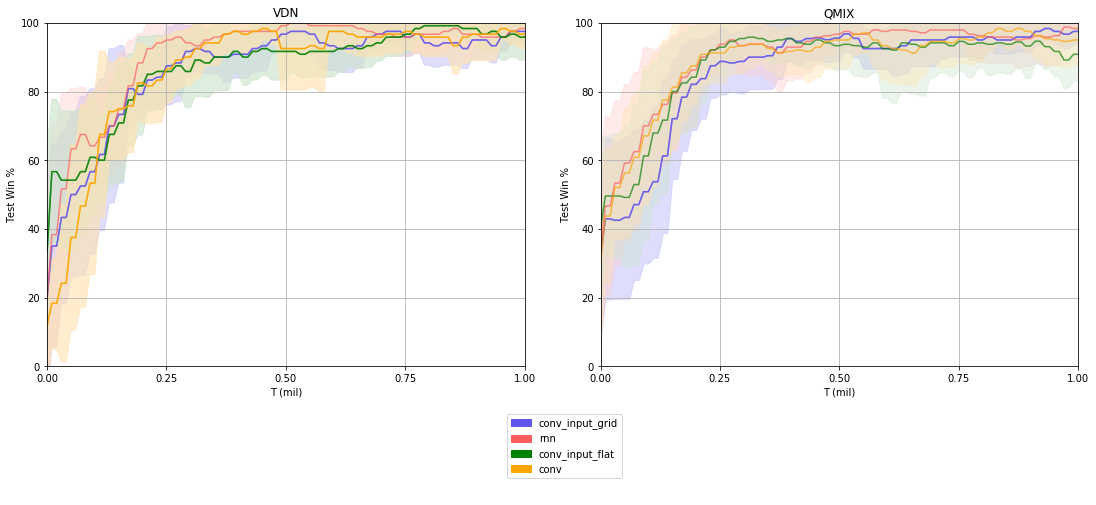
\includegraphics[width=1.34\textwidth]{images/graphs/all3m.png}}
    \caption{Mean test win rate of different architectures on the 3m map. The shaded region shows one standard deviation above and below the mean.}
    \label{fig:3m_all}
\end{figure}

\subsubsection{Baseline Experiments on 2s3z}
We now perform the same baseline experiments on the 2s3z map. The results of this experiment (for both the VDN and QMIX mixing networks) can be seen in figure \ref{fig:2s3z_all}.

Using the VDN mixing network, we can see both the conv and conv\_input\_flat architectures under perform compared to the standard rnn architecture, while the conv\_input\_grid architecture outperforms it. This suggests that grid based actions as inputs are extremely useful to an agent than grid based observations, and provide a superior insight into its environment.


Using the QMIX mixing network, performance was high on all architectures: each exhibited a large limit win rate and fast convergence. However, we clearly see that both the conv and conv\_input\_flat architectures unde-performed compared to the standard rnn network. This suggests that, in a more complex map with multiple types of units (such as 2s3z), if an architecture is using a convolutional encoder for grid based observations then it needs grid based actions as inputs to be effective. 

There was increased variance in the performance on the 2s3z map when compared to the 3m map. This is likely due to the grid representation of observations, and the number different of units: the relationships between the agents (and enemies) is harder to capture on this map.

\begin{figure}[h]
    \centering
    \hbox{\hspace{-6.35em}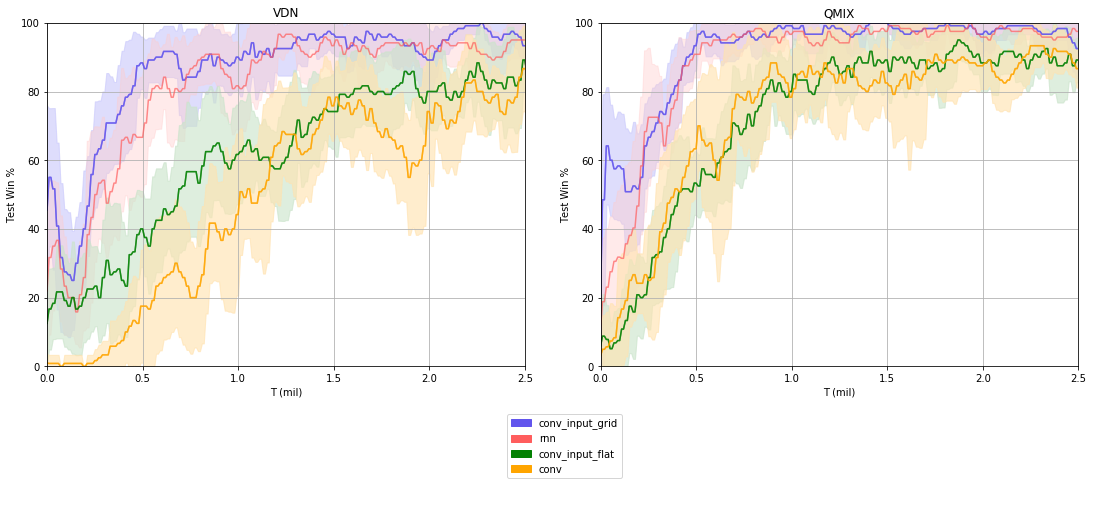
\includegraphics[width=1.34\textwidth]{images/graphs/all2s3z.png}}
    \caption{Mean test win rate of different architectures on the 2s3z map. The shaded region shows one standard deviation above and below the mean.}
    \label{fig:2s3z_all}
\end{figure}





\subsection{Experiments On Different Grid Sizes}
In this section we experiment with different grid sizes for the inputs of conv\_input\_grid (both the observations and actions as inputs). A trade-off is made between the simplicity of a small grid (which has a smaller network that can train more quickly) and the level of detail that can be achieved with a larger grid, allowing for greater spatial relationships to be made between the units. However, larger grids may dilute the data and be unable to extract meaningful information.

The experiments will be performed using the same set up as before, and will take place on the 2s3z map, as this includes units of different types.



The grid sizes we will test are 6x6, 12x12, 18x18 and 24x24. This is because the convolutional encoder kernels (of size 3x3) are simply too large for an input of size smaller than 6x6, and recent tests show that grids larger than 24x24 run out of memory, even with small batch sizes. As described in section 3.4.2, some simple tests were run to find the optimal batch sizes for the different sizes of grid observations. Every other configuration parameter was kept the same for each experiment.





The conv\_input\_grid architecture was experimented upon for each of these grid sizes, with the results shown in figure \ref{fig:gridsizes}.


\begin{figure}
    \centering
    \hbox{\hspace{5em}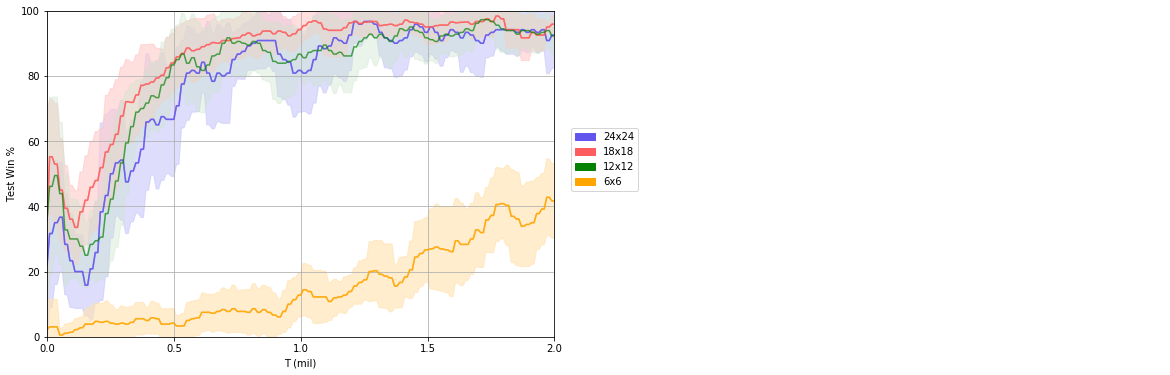
\includegraphics[scale=0.5]{images/graphs/grids.png}}
    \caption{Mean test win rate of the conv\_input\_grid architecture with various grid sizes. The shaded region shows one standard deviation above and below the mean.}
    \label{fig:gridsizes}
\end{figure}

The 12x12, 18x18 and 24x24 grid sizes performed very similarly, each having good performance. Each size has a very large initial rate of learning (between 0 and 200,000 timesteps), reaching around a $50\%$ test win rate very quickly. From here on, every grid size exhibits a steady increase to its convergence of around $92\%$ test win rate after around 3,000,000 timesteps. The similarity of these results suggest that a grid size of $12 \times 12$ or above is enough to represent the environment effectively.

However, some grid sizes have more variance in their performance at different timesteps. For example, the $24 \times 24$ grid (shown in blue in figure \ref{fig:gridsizes}) has the highest variance before convergence. $12 \times 12$ (shown in green) has particularly low variance at this point. On the other hand, the $24 \times 24$ grid exhibits the lowest variance after convergence, whereas the $12 \times 12$ grid has the largest variance in this timeframe. An explanation for this is that the $24 \times 24$ grid was trained with a smaller batch size. This inherently introduces more noise into the gradient descent steps, increasing variance as it is trained. However, once it converges, the size of the grid allows for a very detailed abstraction of the environment, so gives more stable performance.


Clearly, the $6 \times 6$ grid performs very poorly: although some learning can be seen to have taken place, little progress and large variance is still apparent after in comparison to the other sizes. This is likely a result of the grid not being able to represent the complexities of the map well enough: the relations between agents has been abstracted too far away, since 36 cells is not enough to represent this. 

Another suggestion for this lack of performance is the effect of multiple occupancy. On a smaller grid, it is more likely that the multiple occupancy algorithm will be employed, which may have a negative effect on performance, as the observation the agent receives is different from the true observation. In order to see this, we will run a simple test to measure the number of time multiple occupancy occurs over a period of training. Shown in the table below are the average number of cells with multiple occupancy per observation, rounded to two significant figures:


\vspace{3mm}
\begin{center}
\begin{tabular}{ |p{1.8cm}||p{8cm}|  }
 \hline
 \centering Grid Size& \centering Mean Number of Cells With Multiple Occupancy\tabularnewline
 \hline
 \centering 6x6   & \centering 0.65\tabularnewline
 \hline
 \centering 12x12  & \centering 0.25\tabularnewline
 \hline
 \centering 18x18  & \centering 0.18\tabularnewline
 \hline
 \centering 24x24   & \centering 0.0026\tabularnewline
 \hline
 
\end{tabular}
\end{center}
\vspace{3mm}


This makes sense, as the probability of two units occupying the same cell in the grid should decrease in an inverse square fashion, which is similar to what we see here. 

Figure \ref{fig:multocc} shows a comparison of performance between the conv\_input\_grid architecture with and without the resolve multiple occupancy (RSO) algorithm, on both the 6x6 and 12x12 grid sizes. This experiment was performed on the 2s3z map.

\begin{figure}
    \centering
    \hbox{\hspace{5em}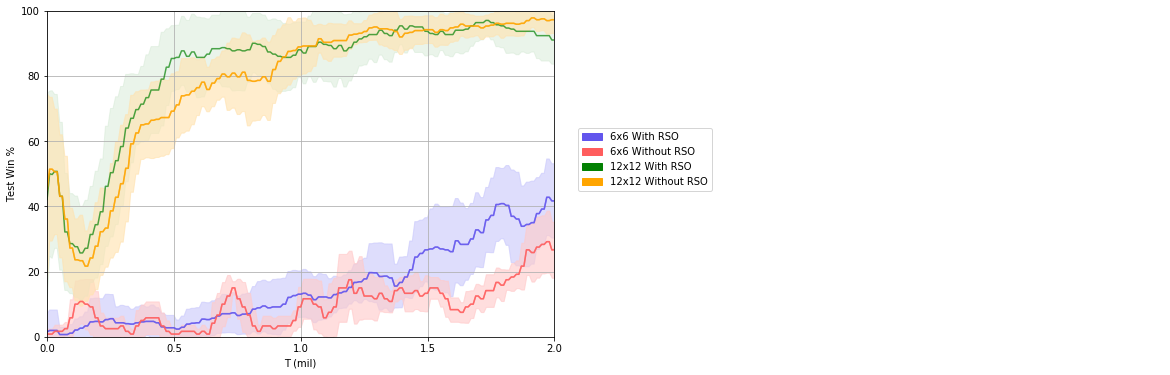
\includegraphics[scale=0.5]{images/graphs/mult_occ.png}}
    \caption{Mean test win rate of the conv\_input\_grid architecture (with various grid sizes) with and without the resolve multiple occupancy (RSO) algorithm. The shaded region shows one standard deviation above and below the mean.}
    \label{fig:multocc}
\end{figure}

As we can see, especially on the 6x6 map, there is some drop in performance when RSO is not used. However, a similar limit performance was reached in both cases. This suggests the algorithm is useful for the network to train, but not essential for good performance. 


\subsection{A Task Invariant Architecture}
In this section we test our central hypothesis that a successful task invariant architecture exists (enabled by the partial observability of StarCraft), particularly with the use of a CNN for the extraction of spatial information.

The conv\_input\_grid architecture is task invariant, except for the input of agent IDs. This is input in order to allow the different agents to share network weights, with the ID being used by the network to distinguish between the agents. However, the RNN and new observation (and action) representation already encode this differentiaiton between agents: the observation is centralised around the agent, and the GRU-cell's `memory' is able to `remember' past observations, making the agents easy to tell apart. Therefore, we hypothesis that the agent ID is a redundant input. We can therefore create a task invariant architecture, conv\_input\_grid\_no\_id, by removing this input.


We now test this hypothesis, using the same experiment set up as before, on both the 3m and 2s3z maps. This allows us to see the effect of removing the agent ID input on both a simple map with one unit type, and a larger map with multiple unit types.

Figure \ref{fig:noid} shows the results of this experiment compared to the previous results for the conv\_input\_grid architecture.

\begin{figure}
    \centering
    \hbox{\hspace{-6.6em}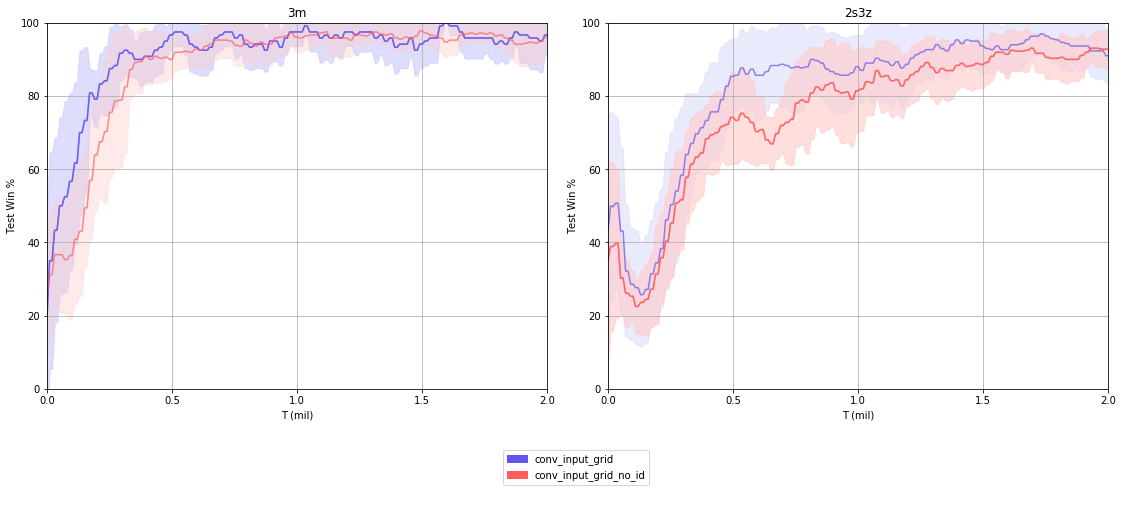
\includegraphics[scale=0.47]{images/graphs/noid.png}}
    \caption{Mean test win rate of the conv\_input\_grid and conv\_input\_grid\_no\_id architectures. The shaded region shows one standard deviation above and below the mean.}
    \label{fig:noid}
\end{figure}


Clearly, the architecture suffered very little decrease in performance on the 3m map. This is expected, as distinguishing agents is not as important on a map with a single unit type: the agents will all simply attack the same enemy for the best results.

Conversely, on the 2s3z map, there was some small decrease in performance, with the conv\_input\_grid\_no\_id architecture taking longer to reach its limit performance. This is explained by the implicit way that the network distinguishes agents, rather than the explicit inputting IDs directly. However, the maximum win rate is still very strong, matching the 95\% exhibited by the original architecture. 


Furthermore, this result allows us to hypothesise that the recurrent nature of the architecture is necessary to distinguish between agents effectively, and therefore exhibit high performance in StarCraft. This is easily tested by removing the GRU-cell from the conv\_input\_grid\_no\_id architecture and performaing the same experiment to measure performance. The result of this experiment is show in figure \ref{fig:rnnvsnonrnn}.

\begin{figure}
    \centering
    \hbox{\hspace{5em}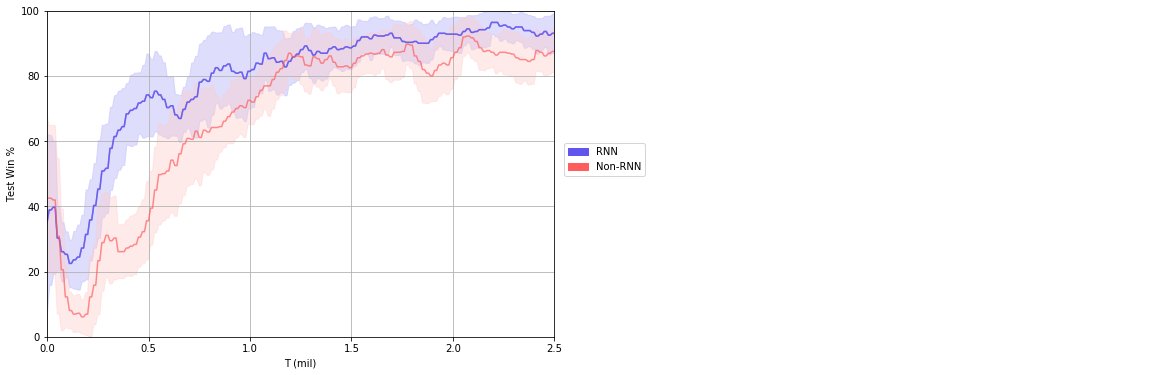
\includegraphics[scale=0.5]{images/graphs/rnn.png}}
    \caption{Mean test win rate of the conv\_input\_grid with and without a GRU-cell before the final linear layer. The shaded region shows one standard deviation above and below the mean.}
    \label{fig:rnnvsnonrnn}
\end{figure}


We can see that, although performance has showed a significant decrease, the network is still learning fairly effectively. Our hypothesis has been shown to be somewhat true, but incomplete: there must be another feature of the architecture that allows it to distinguish between agents and learn effectively. 

The new representation of actions (which are input into the network) may even be rich enough to encode valuable information. Each available action is input into the network (in grid format), with each action being either attack or movement. Whilst the available movement actions generally give little information (an agent can almost always move in any direction), the available attack actions directly inform the network of where the enemies are (since each enemy is a single attack action). We hypothesise that this input is rich enough for high performance.


We run experiments in the same way as before on the conv\_input\_grid\_no\_id architecture. However, we vary the level of observation, from very rich to empty (note that we always pass an available action as an input, so even with an empty observation the network does receive an input). This allows us to clearly see the effect of each observation on performance, as well as to see the base level of performance provided by the input actions.

The level of observations we will use are shown below.

\vspace{3mm}
\begin{center}
\begin{tabular}{|l|l|l|l|l|l|} 
\hline
              & Full & No ID & No ID or Unit Type & Only Ally or Enemy & Empty  \\ 
\hline
Agent ID      &  \centering\checkmark    &       &                    &                    &        \\ 
\hline
Unit Type     &  \centering\checkmark     &  \centering\checkmark      &                    &                    &        \\ 
\hline
Health        & \centering\checkmark      &  \centering\checkmark      & \centering\checkmark                    &                    &        \\ 
\hline
Ally or Enemy &  \centering\checkmark     &  \centering\checkmark      &  \centering\checkmark                   &       \centering\checkmark              &        \\
\hline
\end{tabular}
\end{center}
\vspace{3mm}



The relative performance of the architecture with these level of observations can be seen in figure \ref{fig:obs}. 

\begin{figure}
    \centering
    \hbox{\hspace{5em}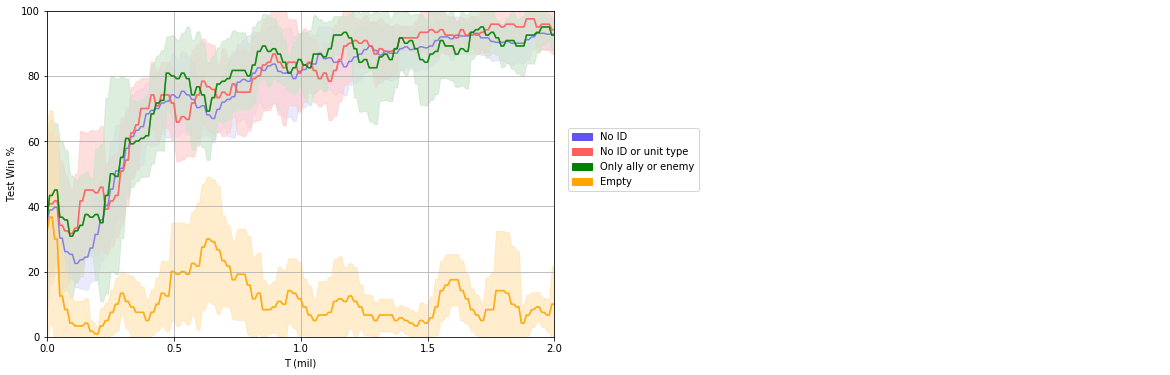
\includegraphics[scale=0.5]{images/graphs/obs.png}}
    \caption{Mean test win rate of the conv\_input\_grid with various levels of observation detail. The shaded region shows one standard deviation above and below the mean.}
    \label{fig:obs}
\end{figure}

As expected, an empty observation gives very poor performance: the network cannot seem to learn at all. Surprisingly, however, every other level of observation showed near identical performance, reaching at least a $95\%$ win rate after just 2 million timesteps. This suggests that the only observation that is necessary in this architecture is ally\_or\-enemy. An explanation for this is the fact that the network can derive very useful information from the input actions, such as enemy locations, but is not able to see allies without the ally\_or\_enemy observation. This prevents teamwork, and leads to uncoordinated, inferior play. 










\subsection{Transfer Learning}

Finally, with our task invariant architecture (conv\_input\_grid\_no\_id) we are able to test our central hypothesis by evaluating the performance of a trained model on a different map.

To start, we will experiment upon transfer learning between the simple (single unit type) maps, 3m, 5m and 8m. We simply take a previously trained model for the relevant map, and begin training this network on another map. We will then compare the performance of this network (which has previously been trained on another map) with a network that was only trained on this map. Initially, we will only experiment with transfer learning between 3m and 5m, and 5m and 8m, to ensure the maps are as similar as possible, in line with our hypothesis.

Under the assumption of our central hypothesis, we should see immediate benefit from having been trained on another map, because (under our hypothesis) the maps look similar due to the partial observability of the agents. Therefore, we expect a network that has been warm-started on another map to initially exhibit superior performance (hopefully close to the maximum win-rate of the network on the map it was trained on) when compared to the standard network.


Firstly, we use a network that has reached the limit of performance for the warm-start of training on a different map. For 3m, 5m and 8m, this is after 600,000 timesteps.


We see in figure \ref{fig:transfer6} that this is not the case. In fact, we see the opposite result in some cases: warm-start training appears to be a disadvantage in some scenarios. In the 3m to 5m transfer case, we see that the network is unable to learn at all until around 200,000 timesteps, while a fresh network learns immediately.

\begin{figure}[h]
    \centering
    \hbox{\hspace{-5em}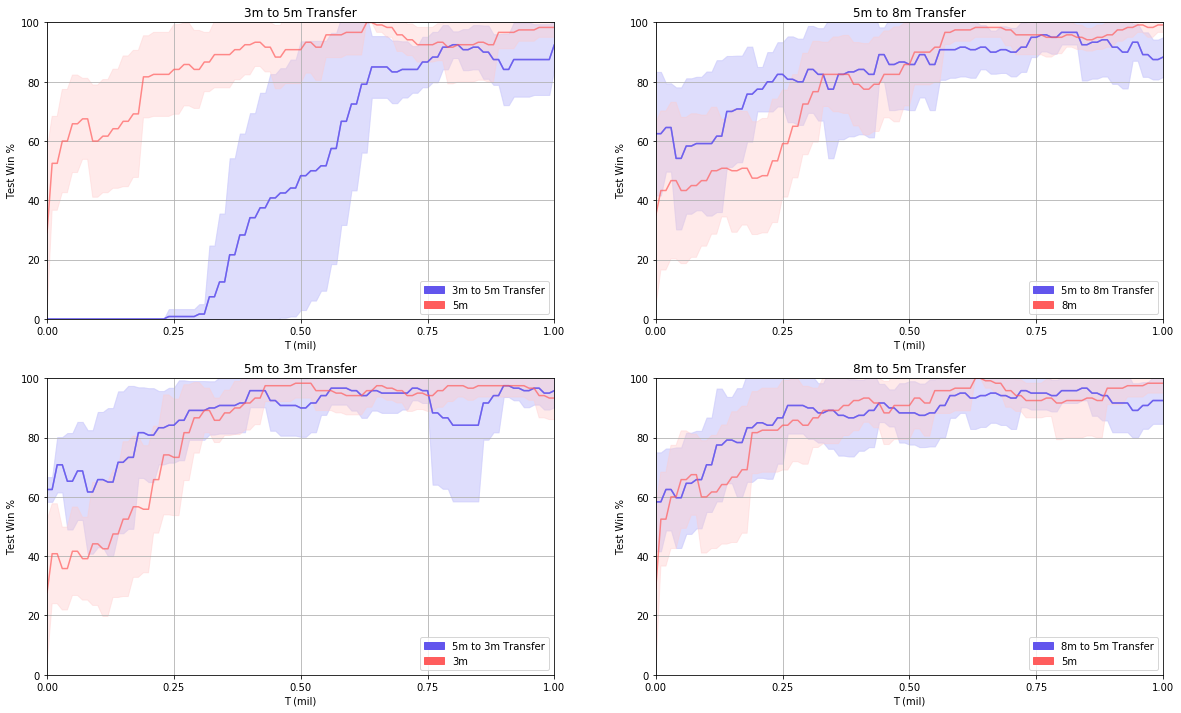
\includegraphics[width=1.2\textwidth]{images/graphs/6.png}}
    \caption{Mean test win rate of the conv\_input\_grid\_no\_id architecture on various scenarios using warm-start training (using a network that has trained already trained for 600,000 timesteps on another scenario). The shaded region shows one standard deviation above and below the mean.}
    \label{fig:transfer6}
\end{figure}


The reason for this may be that the network has over-fitted the original map, and is no longer `plastic' enough to learn on another map. The time where no progress is made in the 3m to 5m transfer example can thus be characterised as a period of `undoing' the previous work, in order to be able to learn on this new map.

To test this, we shall try again with networks that have not yet reached limit performance, but have shown some good progress, which is around 200,000 timesteps. At this point, the network is still very `plastic', and able to adapt to other maps, but still has learned a good insight into the game. This experiment is show in figure \ref{fig:transfer2}.


\begin{figure}[h]
    \centering
    \hbox{\hspace{-5em}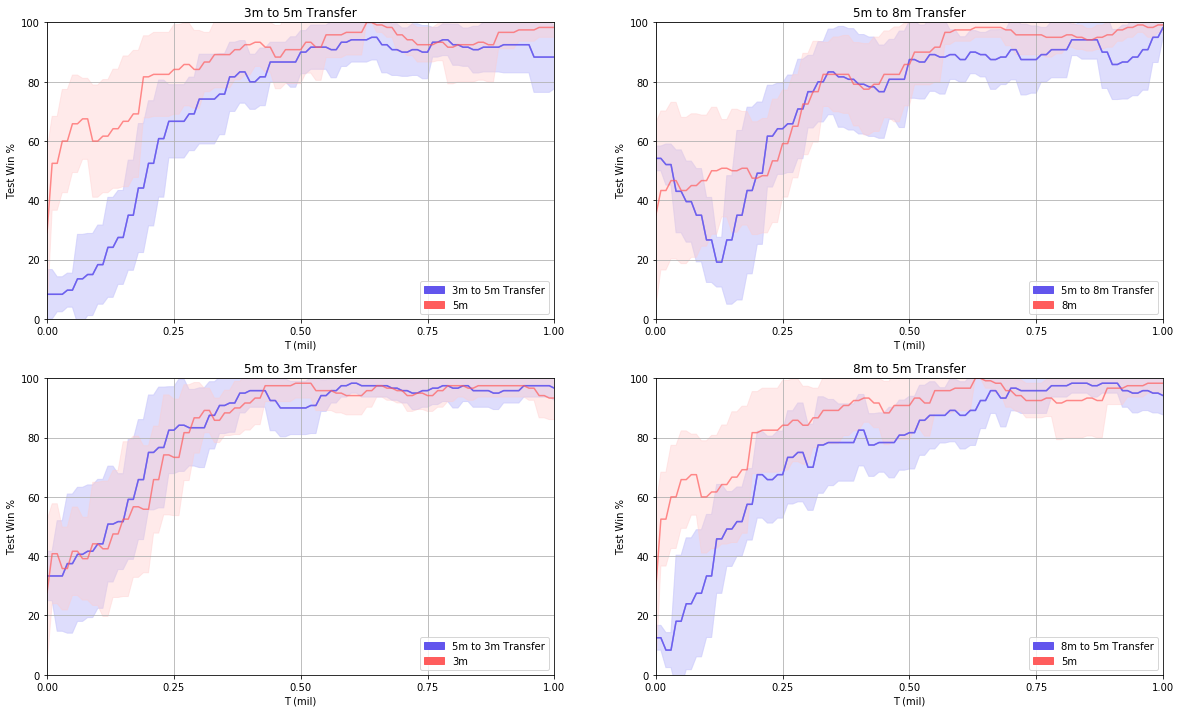
\includegraphics[width=1.2\textwidth]{images/graphs/2.png}}
    \caption{Mean test win rate of the conv\_input\_grid\_no\_id architecture on various scenarios using warm-start training (using a network that has trained already trained for 200,000 timesteps on another scenario).}
    \label{fig:transfer2}
\end{figure}

We see a similar result: the warm-start of training does not provide any benefit. We do see an improvement in the 3m to 5m transfer case, as the network immediately starts to make progress, but it is still far below the performance of a fresh network.

A likely explanation for these results is that the input space is simply too different for a different map. Although the environment is partially observable, agents in different maps will observe a different number or enemies and allies a large amount of the time, especially if the observation radius includes all other enemies (which is very likely during the later, more important stages of the battle). 

Hence, we devise a strategy for a network to learn on multiple maps simultaneously, to enrich the input space and allow for a more generalisable network. We maintain a network during training, and for each episode, we choose a map uniformly at random from a set of available maps, and train as normal. We will start with learning on just two maps, 3m and 5m.

The results of this simultaneous learning can be seen in the top left graph in figure \ref{fig:reptileall}. 




\begin{figure}[h]
    \centering
    \hbox{\hspace{-5em}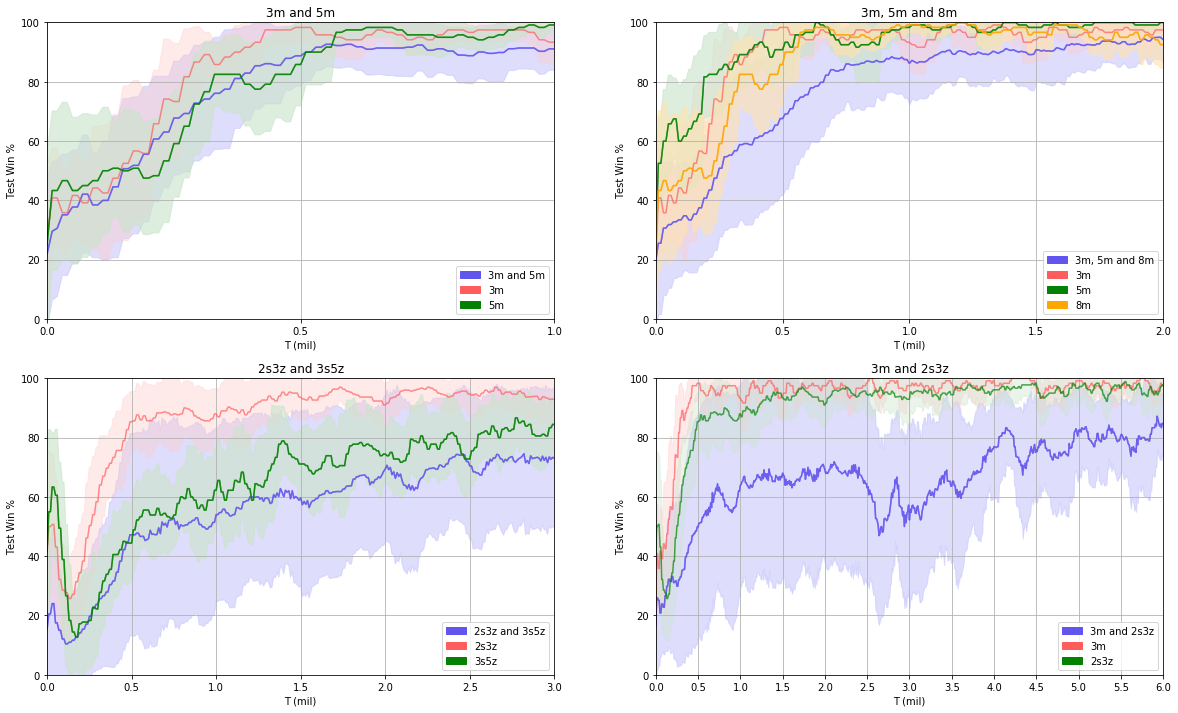
\includegraphics[width=1.2\textwidth]{images/graphs/all.png}}
    \caption{Mean test win rate of the conv\_input\_grid and architecture simultaneously learning various sets of maps simultaneously (tests are performed on a single map chosen uniformly at random at each test interval). The shaded region shows one standard deviation above and below the mean.}
    \label{fig:reptileall}
\end{figure}


We are able to take the resulting network and play with excellent performance on both the 3m and 5m maps individually. 

A natural extension to this experiment is to try to learn on more than 2 maps, or maps with more than one unit type. We therefore run two more experiments: one experiment on 3m, 5m and 8m, and one experiment on 2s3z and 3s5z. The results of these experiments are also shown in figure \ref{fig:reptileall}.



When trained on 3m, 5m and 8m, we can see only a small drop in performance and increase in variance when compared to the performance of training on the individual maps. A similar observation can be made when trained on 2s3z and 3s5z. The performance limit and final variance is equal to those individual maps, showing that, with enough training time, the network can achieve the highest performance possible on multiple maps.

When trained on both 3m and 2s3z, we see a significant decrease in performance when compared to the performance of training on the individual maps. This is likely because each map has an entirely different set of unit types, and therefore the maps are not very similar.

Overall, we have shown that our task invariant architecture is able to learn across various tasks with great success, owing to the similarity of such tasks, thus proving our central hypothesis.